\documentclass{beamer}
\mode<presentation>
\usepackage{amsmath}
\usepackage{amssymb}
%\usepackage{advdate}
\usepackage{adjustbox}
\usepackage{subcaption}
\usepackage{enumitem}
\usepackage{multicol}
\usepackage{mathtools}
\usepackage{listings}
\usepackage{url}
\def\UrlBreaks{\do\/\do-}
\usetheme{Boadilla}
\usecolortheme{lily}
\setbeamertemplate{footline}
{
  \leavevmode%
  \hbox{%
  \begin{beamercolorbox}[wd=\paperwidth,ht=2.25ex,dp=1ex,right]{author in head/foot}%
    \insertframenumber{} / \inserttotalframenumber\hspace*{2ex} 
  \end{beamercolorbox}}%
  \vskip0pt%
}
\setbeamertemplate{navigation symbols}{}

\providecommand{\nCr}[2]{\,^{#1}C_{#2}} % nCr
\providecommand{\nPr}[2]{\,^{#1}P_{#2}} % nPr
\providecommand{\mbf}{\mathbf}
\providecommand{\pr}[1]{\ensuremath{\Pr\left(#1\right)}}
\providecommand{\qfunc}[1]{\ensuremath{Q\left(#1\right)}}
\providecommand{\sbrak}[1]{\ensuremath{{}\left[#1\right]}}
\providecommand{\lsbrak}[1]{\ensuremath{{}\left[#1\right.}}
\providecommand{\rsbrak}[1]{\ensuremath{{}\left.#1\right]}}
\providecommand{\brak}[1]{\ensuremath{\left(#1\right)}}
\providecommand{\lbrak}[1]{\ensuremath{\left(#1\right.}}
\providecommand{\rbrak}[1]{\ensuremath{\left.#1\right)}}
\providecommand{\cbrak}[1]{\ensuremath{\left\{#1\right\}}}
\providecommand{\lcbrak}[1]{\ensuremath{\left\{#1\right.}}
\providecommand{\rcbrak}[1]{\ensuremath{\left.#1\right\}}}
\theoremstyle{remark}
\newtheorem{rem}{Remark}
\newcommand{\sgn}{\mathop{\mathrm{sgn}}}
\providecommand{\abs}[1]{\left\vert#1\right\vert}
\providecommand{\res}[1]{\Res\displaylimits_{#1}} 
\providecommand{\norm}[1]{\lVert#1\rVert}
\providecommand{\mtx}[1]{\mathbf{#1}}
\providecommand{\mean}[1]{E\left[ #1 \right]}
\providecommand{\fourier}{\overset{\mathcal{F}}{ \rightleftharpoons}}
%\providecommand{\hilbert}{\overset{\mathcal{H}}{ \rightleftharpoons}}
\providecommand{\system}{\overset{\mathcal{H}}{ \longleftrightarrow}}
	%\newcommand{\solution}[2]{\textbf{Solution:}{#1}}
%\newcommand{\solution}{\noindent \textbf{Solution: }}
\providecommand{\dec}[2]{\ensuremath{\overset{#1}{\underset{#2}{\gtrless}}}}
\newcommand{\myvec}[1]{\ensuremath{\begin{pmatrix}#1\end{pmatrix}}}
\let\vec\mathbf

\lstset{
%language=C,
frame=single, 
breaklines=true,
columns=fullflexible
}

\numberwithin{equation}{section}

\title{Presentation}
\author{Mohit \\ EE24BTECH11041}
\date{23 JAN 2025}
\begin{document}

\begin{frame}
\titlepage
\end{frame}

\section*{Outline}
\begin{frame}
\tableofcontents
\end{frame}
\section{Problem}
\begin{frame}
\frametitle{Problem Statement}
%
On comparing the ratios $\frac{a_1}{a_2},\frac{b_1}{b_2}$ and $\frac{c_1}{c_2}$, find out whether the lines representing the following pair of linear equation intersect at a point , are parallel or coincident:\\
\begin{align}
9x + 3y + 12 = 0 \\
18x + 6y + 24 = 0
\end{align}
\end{frame}

\section{Solution}
\subsection{Solution}
\begin{frame}
\frametitle{Solution}


Given,
\begin{align}
a_1=9,b_1=3,c_1=12,a_2=18=b_2=6,c_2=24 \\
\frac{a_1}{a_2}=\frac{b_1}{b_2}=\frac{c_1}{c_2}=\frac{1}{2}
\end{align}
Hence,both lines are same.
    \end{frame}
    

\begin{frame}
\frametitle{LU-Decomposition}

	We rewrite the equations as:
	\begin{align}
		x &= x_1, \\
		y &= x_2,
	\end{align}
	giving the system:
	\begin{align}
		9x_1 + 3x_2 &= -12, \\
		18x_1 + 6x_2 &= -24.
	\end{align}
	
	\textbf{Step 1: Convert to Matrix Form}
	We write the system as:
	\begin{align}
		A \mathbf{x} &= \mathbf{b},
	\end{align}
	where:

\end{frame}

\begin{frame}
\frametitle{LU-Decomposition}


\begin{align}
		A &= \begin{bmatrix} 9 & 3 \\ 18 & 6 \end{bmatrix}, \\
		\mathbf{x} &= \begin{bmatrix} x_1 \\ x_2 \end{bmatrix}, \\
		\mathbf{b} &= \begin{bmatrix} -12 \\ -24 \end{bmatrix}.
	\end{align}
	
    \textbf{Step-by-Step Procedure:}\\
1.Let 
\begin{align}
U= \begin{bmatrix} U_{11} & U_{12} \\ U_{21} & U_{22} \end{bmatrix} \text{ and } L= \begin{bmatrix} 1 & 0 \\ l_{21} & 0 \end{bmatrix}
\end{align}

\end{frame}

\begin{frame}
\frametitle{LU-Decomposition}
  
2. Result:\\
   - After completing the iterations, the matrix $ \mathbf{A} $ is decomposed into $ \mathbf{L} \cdot \mathbf{U} $, where $ \mathbf{L} $ is a lower triangular matrix with ones on the diagonal, and $ \mathbf{U} $ is an upper triangular matrix.

\textbf{1. Update for $ U_{k,j} $ (Entries of $ U $)}

For each column $ j \geq k $, the entries of $ U $ in the $ k $-th row are updated as:

\[
U_{k,j} = A_{k,j} - \sum_{m=1}^{k-1} L_{k,m} \cdot U_{m,j}, \quad \text{for } j \geq k.
\]
This equation computes the elements of the upper triangular matrix $ \mathbf{U} $ by eliminating the lower triangular portion of the matrix.

\end{frame}

\begin{frame}
\frametitle{LU-Decomposition}


\textbf{2. Update for $ L_{i,k} $ (Entries of $ L $)}

For each row $ i > k $, the entries of $ L $ in the $ k $-th column are updated as:
\[
L_{i,k} = \frac{1}{U_{k,k}} \left( A_{i,k} - \sum_{m=1}^{k-1} L_{i,m} \cdot U_{m,k} \right), \quad \text{for } i > k.
\]
This equation computes the elements of the lower triangular matrix $ \mathbf{L} $, where each entry in the column is determined by the values in the rows above it.\\
Using a code we get L,U as 
\begin{align}
    L=\begin{bmatrix} 1 & 0 \\ 2 & 1 \end{bmatrix}
    U=\begin{bmatrix} 9 & 3 \\ 0 & 0 \end{bmatrix}
\end{align}
\end{frame}


\begin{frame}
\frametitle{LU-Decomposition}
\textbf{Step 3: Solve $L\mathbf{y} = \mathbf{b}$ (Forward Substitution)}
	We solve:
	\begin{align}
		L\mathbf{y} = \mathbf{b} \quad \text{or} \quad \begin{bmatrix} 1 & 0 \\ 2 & 1 \end{bmatrix} \begin{bmatrix} y_1 \\ y_2 \end{bmatrix} = \begin{bmatrix} -12 \\ -24 \end{bmatrix}.
	\end{align}
	Thus:
	\begin{align}
		\mathbf{y} &= \begin{bmatrix} -12 \\ 0 \end{bmatrix}.
	\end{align}


	\textbf{Step 4: Solve $U\mathbf{x} = \mathbf{y}$ (Backward Substitution)}
	We solve:
	\begin{align}
		U\mathbf{x} = \mathbf{y} \quad \text{or} \quad \begin{bmatrix} 9 & 3 \\ 0 & 0 \end{bmatrix} \begin{bmatrix} x_1 \\ x_2 \end{bmatrix} = \begin{bmatrix} -12 \\ 0 \end{bmatrix}.\\
	 \begin{bmatrix} 9x_1 + 3x_2 \\ 0 \end{bmatrix} = \begin{bmatrix} -12 \\ 0 \end{bmatrix}.\\
	\end{align}
	Hence ,there exist infinity many values of $x_1$ and $x_2$.
	So, both lines are same.


\end{frame}

\section{Plot}
\subsection{Plot}
\begin{frame}
\frametitle{Plot}


\begin{figure}[h!]
   \centering
   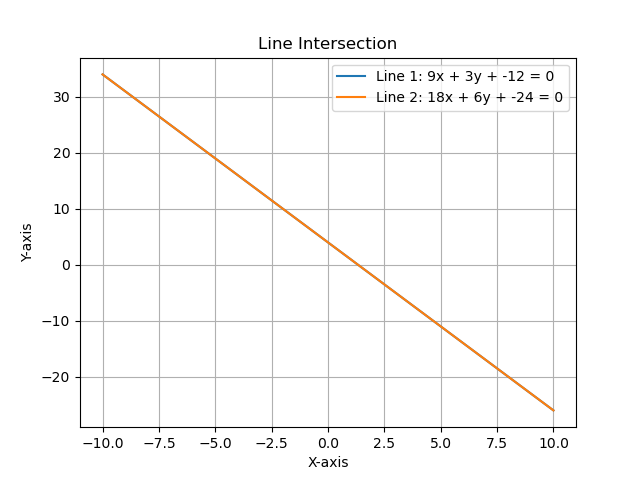
\includegraphics[width=0.7\linewidth]{figs/Figure_1.png}
   \label{Graph by Finite difference Method}
\end{figure}
\end{frame}




\end{document}
